\documentclass[11pt,a4paper]{article}
\usepackage[utf8]{inputenc}
\usepackage[a4paper]{geometry}

\usepackage[english]{babel}
\hyphenation{sil-la-ba-zio-ne pa-ren-te-si}
\usepackage{newlfont}

\usepackage{amsmath}
\usepackage{amsfonts}
\usepackage{amssymb}
\usepackage{amsthm}
\usepackage {amsmath, amssymb} 
\usepackage{bbm}

\usepackage{graphicx}
\usepackage{rotating}
\usepackage{subfigure}
\usepackage{lscape}
\usepackage[bf, scriptsize]{caption}
\usepackage{multirow}
\usepackage{longtable}
\hyphenation{Low-din}
\usepackage{titling}
\usepackage{eurosym}
\usepackage{adjustbox}


\author{F. Cinus \& F. Delussu \& N. Sella}
\title{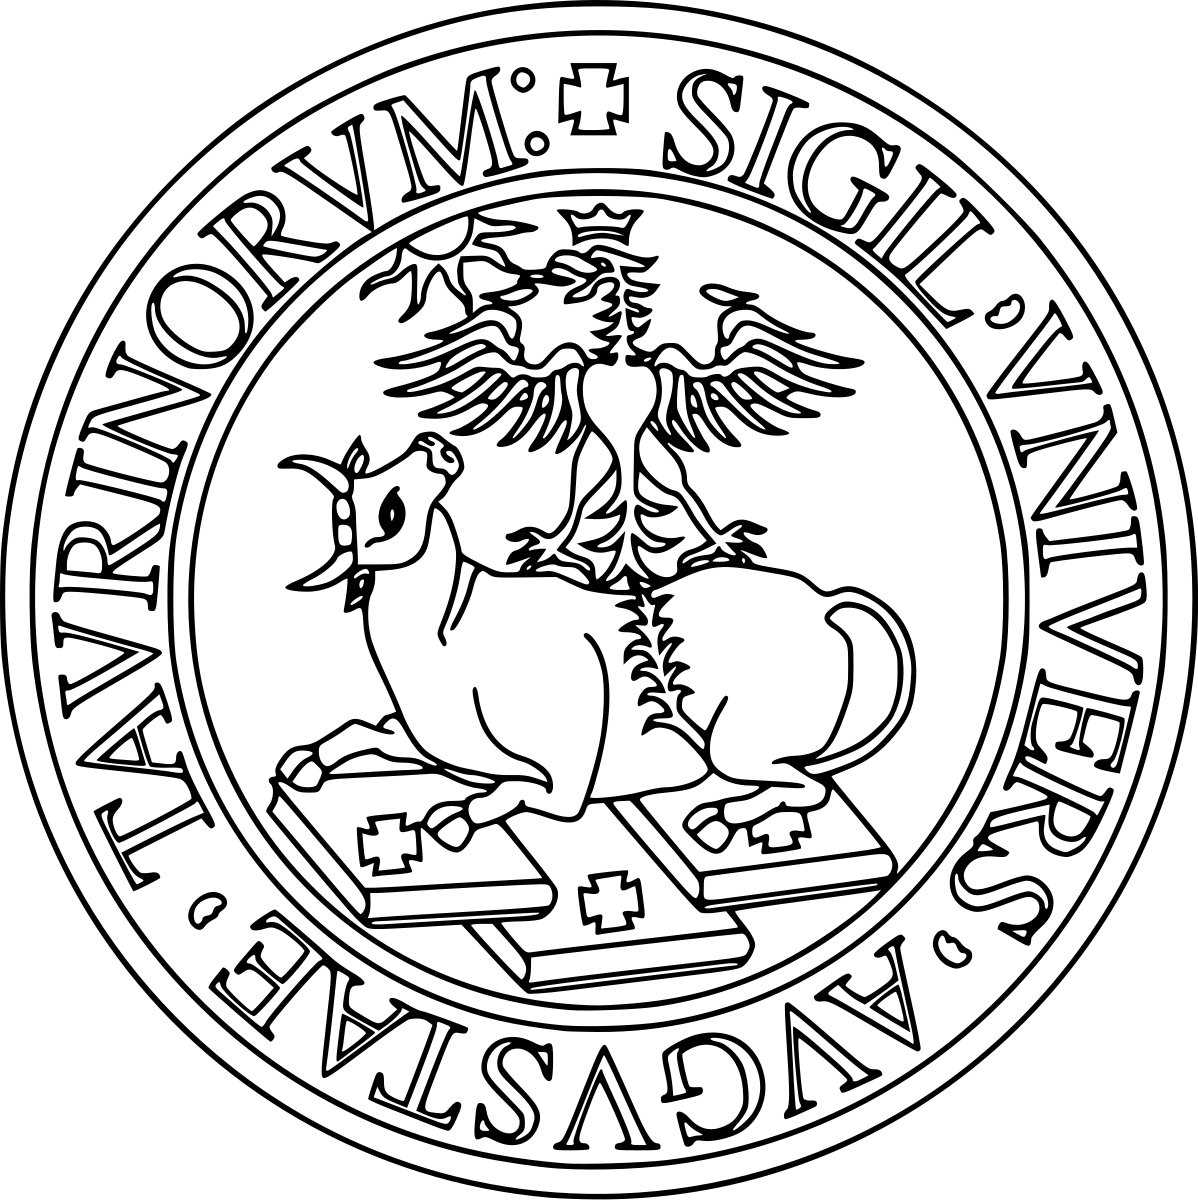
\includegraphics[scale=0.12]{Unito-logo} \\ \LARGE{UNIVERSIT\`{A} DEGLI STUDI DI TORINO} 
\\
TANS Course A.A. 2017/2018 Prof. Massimo Masera
\\
 \textbf{Ising Model Simulation with Monte Carlo methods}
}

\begin{document}
\date{}
\maketitle
\bigskip
\section*{Abstract}
In this work is introduced the Last Mile problem and the Agent-Based modelling process.
A solution for the Last Mile problem is proposed suggesting an active engagement of the population.
Some estimation has been done in order to make the simulation suitable for representing the city of Turin and actual cost of the delivering process.
Results show the robustness of the proposed solution both in economical and user's engagement terms, discussing also extreme situation.

%-----------------------------PAG 1----------------------------------%
\newpage
\section*{Introduction}
The Ising model is a well studied model in Statistical Mechanics which describes ferromagnetism phenomena. It is characterized by a microscopic configuration space based on D-dimensional lattice, that brings to macroscopic statistical quantities. Moreover it can easily generalize the concept of collective effects caused by binary valued points interacting in pairs; for this reason the Ising model became the core of the physics of complex systems. In the last decades computational methods have been applied to search a numerical solution for the 3D Ising model in order to  fill the lack of an analytical solution.  
\\
Alongside Metropolis algorithm became the most popular method of important sampling in MC. The basic idea of a weighted sampling based on the importance of a region determined a great step for the numerical solutions in general. Under these premises we want to outline the purpose this work wants to pursuit: finding numerical solution of the ND-dimensional Ising model with Metropolis algorithm.


\begin{figure}[h!]
\centering
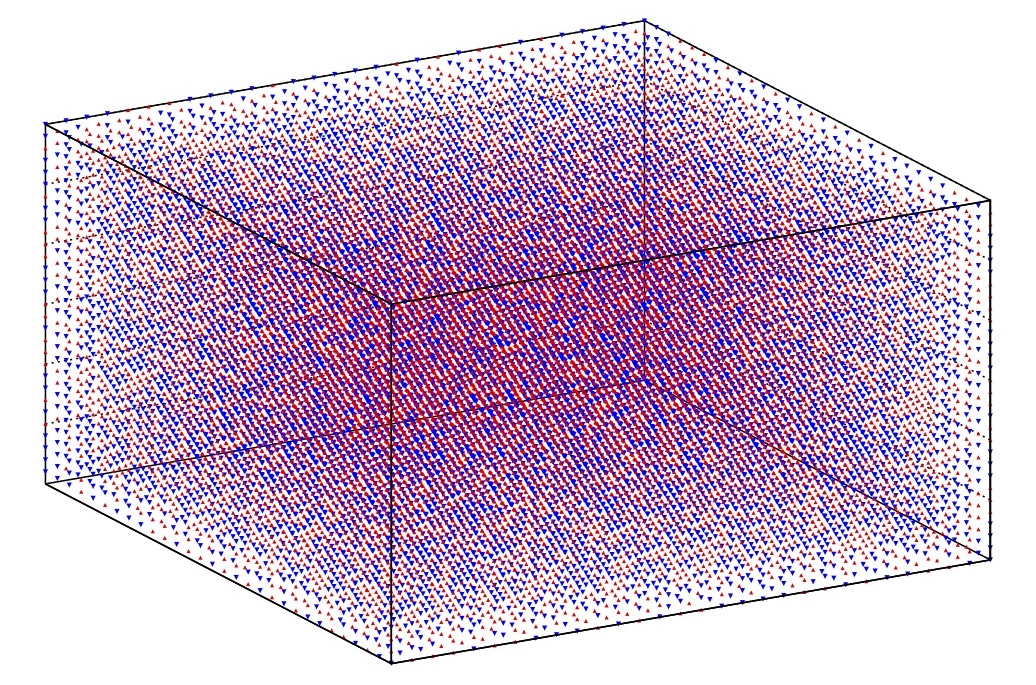
\includegraphics[scale=0.25]{img/img1_intro.jpg} 
\caption[Source: "monteinsing code" https://inknos.github.io/monteising/]{High temperature simulation of 3D Ising model}
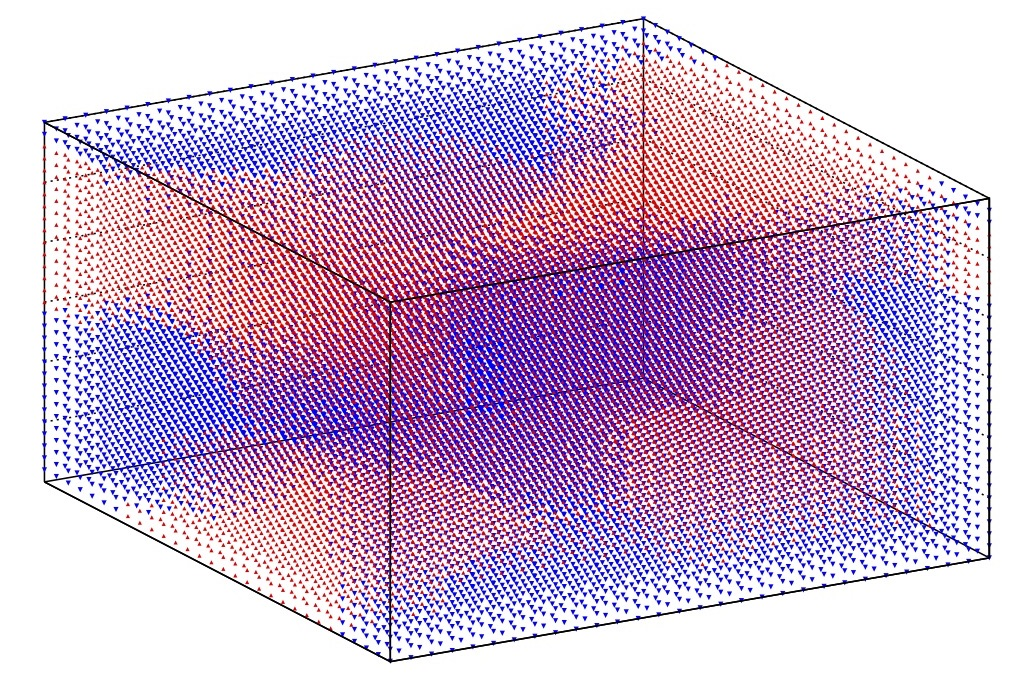
\includegraphics[scale=0.25]{img/img2_intro.jpg} 
\caption[Source: "monteinsing code" https://inknos.github.io/monteising/]{Low temperature simulation of 3D Ising model}
\end{figure}


%-----------------------------PAG 2----------------------------------%
\newpage 
\section{Theory}
\subsection{Ising model and importance sampling}
The Ising model is a physical-mathematical model characterized by a lattice of local spins in the [-1;+1] domain. The correspondent energy is proportional to the quadratic interaction of near spins ($\sigma_i$): 

\begin{equation}
H(q, \sigma) = \sum_{<l,m>}^{'} -J\sigma_i\sigma_j 
\end{equation}
Where $J$ is the energy interaction term and we sum over the neighbours.
\\
The system has  a macroscopic equilibrium state (macrostate) described by statistical quantities: number of spins $N$, lattice volume $V$, energy $E$, magnetization $M$. According to the Statistical Mechanics theory we consider the thermodynamic limit, i.e. $N, V \rightarrow \infty$ and $N/V = cost$ in order to have negligible fluctuations on energy and magnetisation: $(\Delta E)^2 / \langle E \rangle = O  (1/ \sqrt{N}) $.
From a theoretical point of view we consider an ensemble of lattices, each one with a particular configuration of spins (microstate) that corresponds to the same macrostate; we underlying that all microstates are equiprobable. The configuration space is described through the Hamiltonian formalism indeed, under ergodic hypothesis, the system visits all microstates. Moreover stationary hypothesis implies the existence of an equilibrium state in which  the probability distribution of the microstates satisfies the Liouville theorem. These hypotheses bring respectively to the following statements:

\begin{enumerate}
\item In the $t \rightarrow \infty$ limit: the average (over all the ensemble) of a physical quantity is equal to the temporal average of that quantity.
\item The probability distribution of the microstates depends only on the Hamiltonian:
\begin{equation}
\rho (q, \sigma ) \propto \exp \lbrace- \beta H(q, \sigma ) \rbrace 
\end{equation}
Where $q$ is the spin position on the lattice and $\beta$ is the product of the Boltzmann constant and the temperature $T$ of the system.
\end{enumerate}


In a finite case the Ising model system is characterized by magnetization and  energy fluctuations that brings us to consider it under canonical formalism. We define the partition function as follow: $Z = \sum_q exp [  -\beta H(q) ]$. The model simulation can be done through Monte Carlo method, i.e. we generate a pseudo-random chain of numbers in order to extract a microstate sample (from all the configuration space) distributed by the following equilibrium distribution of probability:
\begin{equation}
P_{eq}(q)=\exp \lbrace -\beta H(q)\rbrace /Z
\end{equation} 
In practice we cannot compute the partition function, moreover an algorithm that search over all the phase space has not a great performance. 


%-----------------------------PAG 3----------------------------------%
\newpage
The Boltzmann's factor as probability of choosing a configuration gives a great improvement for the simulation. In this way we are not sampling all the configuration space but a selected and uniform distributed microstates collection. This approach is called \textit{importance sampling} and it allows us to calculate physical quantities as the average number over the extracted configuration:
\begin{equation}
\langle E \rangle_N = \dfrac{1}{N} \sum_{i=1}^{N}{E(q_i)}
\end{equation} This intuition can be proved under ergodic hypothesis: in fact we can consider an evolving Ising system in which there is a spin flip at each time step. The temporal collection of microstates is a Markov chain with a transition probability ($W$) that leads the system to the equilibrium probability in the $t \rightarrow \infty$ limit. Indeed the ratio of the transition probability is:
$$ \dfrac{W(q \rightarrow q')}{W(q' \rightarrow q)} = \dfrac{P_{eq}(q')}{P_{eq}(q)}= \exp \lbrace \beta [E(q) - E(q')] \rbrace $$
Where $q$ and $q'$ are respectively the configuration before the spin-flip and after. This implies the equivalence between importance sampling and random extraction. The arbitrary choose on $W(q \rightarrow q')$ determines the particular algorithm; for the Metropolis-Hastings algorithm:

\begin{eqnarray}
W(q \rightarrow q')=1 \qquad \Delta E \leq 0 \\
W(q \rightarrow q')=\exp \lbrace -\beta \Delta E  \rbrace  \: \Delta E > 0
\end{eqnarray}

\bigskip

\subsection*{Phase transition in Ising model}
Magnetization in Ising model shows phase transition at a certain temperature called $T_c$. This means that the logarithm of the partition function has critical point of the first order in this point and two different statistical descriptions concurrently exist at $T_c$. Indeed the magnetization curve has two different fits before this point and after, that corresponds to inner configuration of spins: random that corresponds to $\langle M \rangle = 0$ and ordered with $\langle M \rangle \rightarrow +1 / -1$. 

 



%-----------------------------PAG 4----------------------------------%
\newpage


%-----------------------------PAG 5----------------------------------%
\newpage 
\section{Code}
This section's aim to introduce a possible solution to the Last Mile Problem that we investigated and modeled. 
The approach to this problem comes from the analysis of the city of Turin, in particular about the urban situation and the world of the sharing economy. 
First of all, as we shown in the introducing section, nowadays every city in the world is growing and becoming (in our terms) more complex, our case study will be Turin. 
This complexity causes inefficiency of transportation in urban area, the lack of mobility, and an increase of pollution. 
All forecasts about those problems  affecting cities are not optimistic and a lot of research is focused on this aspect. 
Starting from those premises we turn our interest on the world of sharing economy watching to:
\begin{center}
\begin{itemize}
\item BlaBlaCar (cars)
\item Enjoy (cars)
\item TOBike (bikes)
\item Foodora (bikes)
\end{itemize}
\end{center}
In particular there are 116 TOBike stations with about 10 bikes for each station and 186 Enjoy's cars in Turin. 
Morover there is 1 subway, 10 trams routes and 112 bus routes used by about 1200 vehicles; adding all the private vehicles for a population of 887,101 citizens we discover a great complexity about the transportation system in Turin. 

The main innovation of our idea is to convert this problem in our solution, finding a way to delivery goods all around the city increasing the efficiency as the complexity of a city grows. 
Basic idea is to deal with the delivery process by entrusting the last mile of the package's journey to people that are moving in town to their destination; this lays the bases for the inclusion of citizens, and their urban movements, in the transportation process transmuting them from passive user to active actor and ensuring the ecology of the process. 

We create a model that simulates people traveling with different vehicles in a space to their destination; each one could change his journey, diverting from the original one, in order to deliver a pack to its destination. 
Every person has a different “inner'' cost that depends on his vehicle and personal interest, this brings to an auction in which the delivery company aim at minimizing the expenses, corresponding to the product of the inner cost and the length of the deviation. 
In order to have a more efficient transportation, packs are located in different magazines in the space, taking inspiration to the 20 Amazon's lockers in Turin; obviously they are put in the nearest magazine to the pack's destination. 
The proportionality between deviation and expense needs an incentives analysis in order to reconcile the minimization of the company and the maximization of the ordinary citizen's benefits while guaranteeing the overall ecological benefits to the city.

\newpage
\subsection{Lattice Description}

The “lattice” array of a D-dimensional cubic Lattice is $\mathbf{L} = (L_0,L_1,..,L_{N^D-1})$.
Let $i$ denote the index of the array, ranging from $0$ to $N^D-1$.\\
Let $i$-$spin$ denote the spin represented by the $L_i$ boolean entry. \\
The cartesian coordinates $\mathbf{a} = (a_0,a_1,..,a_{D-1})$ of the $i$-spin can be computed from index $i$ if a convention is set on the lattice arrangement, which in our model is the following: 
\begin{itemize}
	\item The origin \textit{O} of the D-dimensional space is chosen to be a spin-vertex of the cubic Lattice such that each edge starting from \textit{O} is aligned along one of the D positive directions of the space. 
	\item The distance between each couple of adjacent spins is set to one. 
	\item The spins are indexed starting from increasing the first dimension’s coordinate, than the second and so forth.
\end{itemize}

%FIGURA caso 1 , 2 , 3 dimensionale

\textbf{N.B.} This rules imply that, given a specific spin, each coordinate $a_j$ takes values in range 
$\{0,1,…,N-1\}$. \\ 

\subsection*{Coordinates Computation}

Cases from \textit{D=1} to \textit{D=3} are treated in order to understand and generalize the coordinates’ computation. \\
Before starting, the division $/$ and modulo $\%$ operators are defined as follows : \\
Given two integer numbers a and n , the operations a/n and a\%n return respectively the quotient and the remainder of the euclidean division of a by n. \\ 
\textit{e.g.} : $6/3=2$ ; $9/4=2$ ; $6\%3=0$ ; $9\%4=1$ \\

\vspace{0.1cm} 
\textbf{D=1} \\
A 1-dimensional lattice is made by $N$ spins aligned along a single $x$ direction .
In this case the index $i$ represents itself the $x$ coordinate of the spin.\\
%image 1D

\textbf{D=2} \\
A 2-dimensional Lattice is a square made by $N^2$ spins.\\
The index can be expressed as $i = a_0 + a_1N$. \\
$a_1$ can be seen as the number of $N$-spin lines stacked starting from the quote $y=0$, this number is
the $y$-cordinate itself while the number or remaining spin $a_0$ is the $x$-coordinate. 
$a_1$ is computed from $i$ divided by $N$ while $a_0$ is computed from $i$ modulo $N$.
The $(x,y)$ coordinates of the $i$-spin are given by : $$(a_0,a_1)=(i\%N ; i/N)$$ 


\textbf{D=3} \\
A 3-dimensional Lattice is a cube made by $N^{3}$ spins. \\  
The index $i$ can be expressed as $i = a_0 + a_1N + a_2N^2$. \\
$a_2$ can be seen as the number of $N^2$-spin squares stacked starting from the plane $z=0$, this number is 
the $z$ coordinate itself. $a_2$ is computed from $i/N$.
Once we have $a_2$ the remaining $(x,y)$ coordinates can be computed from \\ $i\%N^2 = a_0 + a_1N$ as in \{D=2\} case .\\
The $(x,y,z)$ coordinates of the $i$-spin are given by : $$(a_0,a_1,a_2)=\left( (i\%N^2)\%N , (i\%N^2)/N , i/N^2 \right)$$ 

Generalizing to $D$ dimensions, index $i$ can be expressed as :$ i = \sum_{j=1}^{D-1}a_jN^j $ \\
Its corresponding coordinates are computed starting from $j=D-1$ and establishing a recurrence relationship :
$$\mathbf{a} = \left(a_0 = i\%N ,.., a_j = [i\%N^{j+1}]/N^j ,.., a_{D-2} = [i\% N^{D-1}]/N^{D-2} , a_{D-1} = i/N^{D-1}\right)$$ 
 
\section*{Lattice's energy } 

The Lattice's energy is computed according to : 
$$H = \sum_{<l,m>}^{} -J\sigma_i\sigma_j $$

J is a constant interaction term between each couple $<l,m>$ of spins .\\
The summation is performed over all possible couples $<l,m>$ of adjacent spins.\\

The Lattice class provides a method wich returns the energy of the system. \\
The method's implemented algorithm takes the lattice array and performs two for loops, one over the system's dimension $d = (0,1,..,D-1)$ and the other over the lattice array's index $i = (0,1,..,N^D-1)$. \\
The key idea is that, given a fixed $i$-spin, along each dimension $d$ two neighbours $i_{d_\pm}$-spin are found on the increasing and decreasing d-coordinate respectively. 
\\So each single spin has $2D$ interacting neighbours in total, by summing up their energy interaction terms the contribute of the single spin to the total energy is obtained. So the energy can be rewritten as : 

$$H = \frac{1}{2}\sum_{i=0}^{N^D-1}\sum_{d=0}^{D-1}\sum_{\pm}^{} -J\sigma_i\sigma_{i_{d_\pm}}$$ 

It's easy to observe that, performing the first summation $\sum_{i}^{}$ , double countings of couples occur and a factor $1/2$ is required. \\ 
For each fixed index $i$ ,the algorithm takes into account only the interaction term with the 
$i_{d_+}$-spin so that the number of operation is halved. So the algorithm performs the summation :
  
$$H = \sum_{i=0}^{N^D-1}\sum_{d=0}^{D-1}-J(L_i \ \hat{} \ L_{i_{d_+}})$$ 

$\sigma_i\sigma_{i_{d_+}}$ has been replaced by $L_i \ \hat{} \ L_{i_{d_+}}$ , the former can take values $\pm1$ wether the two spins are aligned or not. Since spins are represented by boolean entries of array $\mathbf{L}$, the XOR bitwise operator $\hat{}$ is applied on couple $(L_i,L_{i_{d_+}})$ so that it returns the same value of $\sigma_i\sigma_{i_{d_+}}$. \\   
\vspace{0.1cm}
From the $i$ index coordinates $\mathbf{a} = (a_0,a_1,..,a_{D-1})$ the $i_{d_+}$ index coordinates 
$\mathbf{a^{d_+}} = (a^{d_+}_0,a^{d_+}_1,..,a^{d_+}_{D-1})$ can be computed. \\
The vector $\mathbf{a^{d_+}}$ differs from $\mathbf{a}$
only on the $d\deg$ entry $a^{d_+}_d$ which is the only one to be increased, this is computed as $(a_d+1)\%N$ since we are applying periodic boundary conditions on the Lattice. 

From this formulas we can express the $i_{d_+}$ index as the sum of two terms:
\begin{eqnarray*}
i_{d_+} &=& \left\{ \sum_{j = 0}^{d-1}a_jN^j  [(a_d + 1)\%N]N^d \right\} + \left\{ \sum_{j = d+1}^{D-1}a_jN^j \right\}  \\
&=& \left\{(i + N^d)\%N^{d+1} \right\}  +  \left\{ (i/N^{d+1})N^{d+1}  \right\} 
\end{eqnarray*}

The algorithm defines two powers \textsf{pow\textunderscore tmp1} and \textsf{pow\textunderscore tmp2}, keeping a fixed index $i$ and performing the loop over d, these powers are assigned respectively to $N^d$ and $N^{d+1}$ in each iteration. 

%-----------------------------PAG 6----------------------------------%
\newpage 
\section{Code}
The basic idea of this work is to give the possibility to every one is traveling in the city to transport a pack to its destination. 
This is a simple concept that, as we shown in the previous section, has some implications. In order to introduce the code to the reader it is useful to present the simulation through its evolution, i.e. we want to show how the code has changed starting from the first idea/solution for the Last Mile Problem to its generalization. 
We remind that the code is written in NetLogo 6.0 and it is possible to freely download it and run the simulation.


\subsection{Moving agents in a cartesian coordinate system}
First of all we have to implement a code that simulates the movement of a defined number of agents in a environment characterized by an empty cartesian coordinate system. 

\begin{figure}[h!]
\centering
%\includegraphics[scale=0.44]{3_1}  
\caption{Moving agents and fixed storages}
\end{figure}

\subsubsection*{Basic Agents}
The basic agent in our simulation will be a breed called “user" moving freely.
They will have a set of own variable, at this point only the destination.
Agents are created in random patches ad are assigned other random patches as destination.
Each agent will then move toward their destination in a straight line and die once reached it.
To avoid the extinction of users, a new one is created in the patch the previous one died.

\subsubsection*{Special Patches}
A special patchset is created to represent the storages around the city.
These patches will be identified by a boolean value, indicating the role of storage or not, and, if so, they will also own a variable “space", that will be further used to represent the physical space in a storage room.
\looseness=-1

\newpage
\subsection{Moving packs}
Once create the basic structure we need to simulate the transportation of packages around the city done by users.
\medskip
\begin{figure}[h!]
\centering
%\includegraphics[scale=0.5]{3_2}  
\caption{Agents delivering packs}
\end{figure}
\medskip
\subsubsection*{Packages}
A breed called “packages" is created in order to simulate the goods transported in the space. Each package will own two variable, one for the destination and another, boolean, to indicate if they are assigned to a user or not.
Each packages is placed in a locker-patch ad assigned a random point on the map as destination.

\medskip
\subsubsection*{Pick-up}
In order to be picked up a package needs to be put in relation with a user.
At first this will be done randomly, the user will go from his position to the position of the package, then do the destination of the package and lastly to his own destination.
To properly keep track of what a user is doing we need to add two new variables to the user breed, “busy" and “bag". Bag will contain the id of the assigned pack and busy will be true if the pack is being transported to its destination by the user.

\newpage
\subsection{Optimizing}
Since now all operation are done randomly and with no regards to the optimization of the process. We need to introduce a way to properly choose the package-user couple such that the distance traveled is minimal.

\begin{figure}[h!]
\centering
%\includegraphics[scale=0.39]{3_3}  
\caption{Cost evolution after auction}
\end{figure}
\subsubsection*{Auction}
To optimize the travel we will use an auction for each package.
Each user will have a new variable, “cost", that will be the amount of a virtual money needed to be paid in order to deviate one patch off the straight line connecting the origin and the destination of the user.
Each package will ask all the user the amount they will need in order to deviate from their original route, pick them up and bring them to destination: the lower bidder will be assigned the pack and will proceed with the delivery.
\begin{figure}[h!]
\centering
%\includegraphics[scale=0.45]{auction}  
\end{figure}
\looseness=-1
\newpage
\subsection{Making it real}
At this point we already have all the essential part of our simulation: agent moving around, delivering packs, in a sort of optimized process. Yet we are far from real and some elements need to be taken into account.

\begin{figure}[h!]
\centering
%\includegraphics[scale=0.4]{3_4}  
\caption{Complex movement behaviour}
\end{figure}
\medskip
\subsubsection*{Highest cost}
The commissioner will not be willing to pay any amount to have his packages delivered, a maximum cost per package is fixed, if the lowest bidder ask for a total amount higher than the fixed maximum cost, the package is not assigned and the auction run again.
\medskip
\subsubsection*{Goods placement}
Packages are not placed randomly in the storages patches but, if the space is enough, each package will be placed in the storage nearest to its destination.

\begin{figure}[h!]
\centering
%\includegraphics[scale=0.77]{place_pack}  
\end{figure}
\newpage
\subsubsection*{Day and night}
People fluxes are not constant during the day, in a city they follow the home-work path one way or the other in the morning and in the evening.
To simulate that we suppose that after a certain amount of ticks we switch from morning to evening.
The cartesian space is divided in two section, the left and the right one respectively along the xcor, during one part of the day agent will be assigned a destination on one side with an higher probability, the other way round during the other part of the day.

\begin{figure}[h!]
\centering
%\includegraphics[scale=0.8]{dest_day_night}  
\end{figure}

\subsubsection*{Randomness}
Random behaviour are created for user: they may, with a small probability, not accept to deliver a package, their internal cost is uniformly distributed around a mean value instead of being fixed.

\subsubsection*{Maintenance cost}
As we can expect the maintenance of all storages around the city will have a cost, more and bigger storages will cost more and add up to the expenses of the commissioner. A value can be chosen to simulate this cost.

\subsection{City of Turin}
In order to scale the simulation to the city of Turin, a series of metric are calculated with the same ratio we can find in the real life, as explained in the previous chapter.

\begin{figure}[h!]
\centering
%\includegraphics[scale=0.8]{scaling}  
\end{figure}

\newpage
\section{Results}
In this section we present the results obtained from the Agent-Based simulation. We discovered that the solution is feasible i.e. people traveling in the city can deliver all packs on time and with a total expense that is lower than the upper-bound (1.75\euro{} per pack). Moreover, being the Foodora's employee salary about 0.5\euro{}/km, we can see that in our estimated range of parameters a person can be paid more than a common delivery man.

Using genetic algorithms implemented in Behavior Search 6.0 we optimized the number of storages and their space, keeping all other estimated parameters fixed such as the number of users, the number of packs and the cost of each box in the storage. 

Figure below show the fitness minimization (expenses) with the following parameters: 1400 packs, 700 users, 1\euro{}/km for users' deviation, 1.75\euro{} as maximum expense for a pack delivery, 0.2\euro{} cost storage's box.

\begin{figure}[h!]
\centering
%\includegraphics[scale=0.33]{BS-02lcost-10lmax-lspace304} 
\caption{Behavior Search result: 10 storages with 304 boxes each, total expense 1439.28}
\end{figure}

Considering 0.8\euro{} as storage's box cost, we find again that the number of boxes in each storage is greater than the minimum needed. This implies that spending money for having bigger storage is useful in case a pack has to be delivered in the neighborhood.

\begin{figure}[h!]
\centering
%\includegraphics[scale=0.33]{BS-08lcost-10lmax-153lspace.png} 
\caption{Behavior Search result: 10 storages with 153 boxes each, total expense 1542.02}
\end{figure}

\newpage 
May be found interesting for the reader to have a deeper look at two of the most important curves in our simulation: number packs vs. time and total expenses vs. time. 

The figure below show that the number of packs exponentially decreases with time as expected.

\begin{figure}[h!]
\centering
%\includegraphics[scale=0.59]{Grafici/Packs(02lcost_10lmax_304lspace).png} 
\caption{Numb packs vs. ticks (10 storages with 304 boxes each, 1400 packs, 700 users)}
\end{figure}

In order to roughly estimate the curve decrease we did a linear regression with 0.07 mean squared error.

\begin{figure}[h!]
\centering
%\includegraphics[scale=0.59]{Grafici/Packs(02lcost_10lmax_304lspace)[E_0,07].png} 
\caption{Fit: numb packs vs. ticks (10 storages with 304 boxes each, 1400 packs, 700 users)}
\end{figure}

\newpage
On the other hand the total expenses approximately increase as a logarithm, which compensates the number of packs trend.

\begin{figure}[h!]
\centering
%\includegraphics[scale=0.6]{Grafici/Total_expense(02lcost_10lmax_304lspace).png}  
\caption{Total expenses vs. ticks (10 storages with 304 boxes each, 1400 packs, 700 users)}
\end{figure}

Even if the mean squared error is considerably worse than the first fitting, we can have an estimate of the curve slope.

\begin{figure}[h!]
\centering
%\includegraphics[scale=0.6]{Grafici/Total_expense(02lcost_10lmax_304lspace)[E_4272].png}  
\caption{Fit: total expenses vs. ticks (10 storages with 304 boxes each, 1400 packs, 700 users)}
\end{figure}

\newpage
At any instant we have a different average cost of delivery, so we can plot the ratio between expenses and packs vs. time. As shown in the figure below the initial costs are relevant but they decrease rapidly with time.

\begin{figure}[h!]
\centering
%\includegraphics[scale=0.8]{Grafici/Total_expense_Packs(02lcost_10lmax_304lspace).png}   
\caption{Total expenses/numb packs vs. ticks (10 storages with 304 boxes each, 1400 packs, 700 users)}
\end{figure}
 
\newpage
\section{Extreme Cases}
As a proof of concept we decided to analyze some extreme cases in order to explore if our solution is robust enough to survive real-life challenges.

\subsubsection*{Too few}
What would happen if there are too few users? 
Keeping all other parameters as found we set the number of users to one tenth the original value, down to 70 agents total.
We observe that the delivery process takes up to two days, instead of the half day in standard situation and the total expenses increase up to 28\% more.



We can have an estimate of the curve slope in log-lin scale.



\newpage
\subsubsection*{Too many}
On the opposite we explore what happens if there are too many users, up to 7000 agents total.
As can be expected the delivery process is completed in a risible time and the expenses are down 70\%, proving the benefit for the commissioner in expanding the participation.


We can have an estimate of the curve slope in log-lin scale.



\newpage
\subsubsection*{Wanting more}
A reasonable question may that an higher pay may be needed to incentive users to participate in the activity. 
We examined what would happen if the pay was up to 5\euro{}/km of deviation.
Similarly to the first case, the process of delivering all packs may take up to two days, but the total expenses will not be too different than the standard situation.


We can have an estimate of the curve slope in log-lin scale.



\newpage
\subsubsection*{High Maintenance}
A success of our method may have the downside of increasing maintenance costs for the storages around the city.
Examining a bi-daily maintenance cost five time the standard situation we found an increase in the total expenses around 21\%, like the first case examined, but without any other downside.



We can have an estimate of the curve slope in log-lin scale.



\newpage
\section{Conclusions}
This work has analyzed a new solution for the LMP characterized by the delivery process carried out by citizens. As we shown in the first section, the today city complexity brought a proportional increase of the transportation costs in it; indeed the presented solution, based on the sharing economy, can be ecologically and economically sustainable. Citizen becomes active actors in the transportation process delivering packs all around the city. The Agent-Based Model has been realized with a scaled map in order to express the Turin's distances and adequate (from a computational point of view) parameters: 
\begin{center}
\begin{tabular}{c|c|c|c|c}
 \hline 
 Numb. Packs & Numb. Users & Max Delivery Cost & Storage Box Cost & Users' Pay \\ 
 \hline 
 \hline
 1400 & 700 & 1.75 \euro{} & 0.2 \euro{}/two days & 1 \euro{}/km \\ 
 \hline 
\end{tabular} 
\end{center} 
The code has been written in NetLogo 6.0 and, thanks to the Behavior Search tool, brought the following results for parameters we need in order to minimize the expenses: 
\begin{center}
\framebox[12cm]{%
 \begin{minipage}{100mm}
 \begin{itemize}
 \item 10 Storages.
 \item 304 Boxes in each storage.
 \item Total expenses: 1440 \euro{}
 \end{itemize}
 \end{minipage}}
 \end{center}
Note that the storage's capacity is greater than the minimum required for an uniform distribution of 1400 packs in 10 storages. This shows how the complex system achieves a store optimization for minimizing the expense regarding random place of delivery.
\bigskip

The figure below shows that the curves of expenses and number of packs vs. time have almost an opposite trend; moreover on the right we see that the expenses for each pack decreases with time.

\newpage
Considering an high and a low number of users we saw that the convergence is faster in the first case and, as expected, less expensive. Note that at the end of the day (1600 ticks) in both cases all packs are delivered.


Increasing the fixed cost parameters we saw that expenses grew, but the model still succeed in delivering all packs in a day (1600 ticks) with a cost for each pack that is lower than 1.75\euro{}.
\\
In conclusion this underlines the robustness of the proposed solution both in economical and user's engagement terms, moreover the model held interesting results also in extreme cases. 

\subsection*{Further development}
The model could be extended by considering:
\begin{itemize}
\item improved economic model;
\item GIS map of the city of Turin;
\item daily data for a real time calculation.
\end{itemize}
\end{document}
